% Options for packages loaded elsewhere
\PassOptionsToPackage{unicode}{hyperref}
\PassOptionsToPackage{hyphens}{url}
%
\documentclass[
]{article}
\usepackage{lmodern}
\usepackage{amssymb,amsmath}
\usepackage{ifxetex,ifluatex}
\ifnum 0\ifxetex 1\fi\ifluatex 1\fi=0 % if pdftex
  \usepackage[T1]{fontenc}
  \usepackage[utf8]{inputenc}
  \usepackage{textcomp} % provide euro and other symbols
\else % if luatex or xetex
  \usepackage{unicode-math}
  \defaultfontfeatures{Scale=MatchLowercase}
  \defaultfontfeatures[\rmfamily]{Ligatures=TeX,Scale=1}
\fi
% Use upquote if available, for straight quotes in verbatim environments
\IfFileExists{upquote.sty}{\usepackage{upquote}}{}
\IfFileExists{microtype.sty}{% use microtype if available
  \usepackage[]{microtype}
  \UseMicrotypeSet[protrusion]{basicmath} % disable protrusion for tt fonts
}{}
\makeatletter
\@ifundefined{KOMAClassName}{% if non-KOMA class
  \IfFileExists{parskip.sty}{%
    \usepackage{parskip}
  }{% else
    \setlength{\parindent}{0pt}
    \setlength{\parskip}{6pt plus 2pt minus 1pt}}
}{% if KOMA class
  \KOMAoptions{parskip=half}}
\makeatother
\usepackage{xcolor}
\IfFileExists{xurl.sty}{\usepackage{xurl}}{} % add URL line breaks if available
\IfFileExists{bookmark.sty}{\usepackage{bookmark}}{\usepackage{hyperref}}
\hypersetup{
  pdftitle={STAT 547M Project},
  pdfauthor={Diana Lin \& Nima Jamshidi},
  hidelinks,
  pdfcreator={LaTeX via pandoc}}
\urlstyle{same} % disable monospaced font for URLs
\usepackage[margin=1in]{geometry}
\usepackage{longtable,booktabs}
% Correct order of tables after \paragraph or \subparagraph
\usepackage{etoolbox}
\makeatletter
\patchcmd\longtable{\par}{\if@noskipsec\mbox{}\fi\par}{}{}
\makeatother
% Allow footnotes in longtable head/foot
\IfFileExists{footnotehyper.sty}{\usepackage{footnotehyper}}{\usepackage{footnote}}
\makesavenoteenv{longtable}
\usepackage{graphicx,grffile}
\makeatletter
\def\maxwidth{\ifdim\Gin@nat@width>\linewidth\linewidth\else\Gin@nat@width\fi}
\def\maxheight{\ifdim\Gin@nat@height>\textheight\textheight\else\Gin@nat@height\fi}
\makeatother
% Scale images if necessary, so that they will not overflow the page
% margins by default, and it is still possible to overwrite the defaults
% using explicit options in \includegraphics[width, height, ...]{}
\setkeys{Gin}{width=\maxwidth,height=\maxheight,keepaspectratio}
% Set default figure placement to htbp
\makeatletter
\def\fps@figure{htbp}
\makeatother
\setlength{\emergencystretch}{3em} % prevent overfull lines
\providecommand{\tightlist}{%
  \setlength{\itemsep}{0pt}\setlength{\parskip}{0pt}}
\setcounter{secnumdepth}{5}

\title{STAT 547M Project}
\author{Diana Lin \& Nima Jamshidi}
\date{14/03/2020}

\begin{document}
\maketitle

{
\setcounter{tocdepth}{2}
\tableofcontents
}
\hypertarget{introduction}{%
\section{Introduction}\label{introduction}}

The dataset we have chosen to work with is the ``Medical Expenses'' dataset used in the book \href{https://www.amazon.com/Machine-Learning-R-Brett-Lantz/dp/1782162143}{Machine Learning with R}, by Brett Lantz. This dataset was extracted from \href{https://www.kaggle.com/mirichoi0218/insurance/home}{Kaggle} by Github user \href{https://gist.github.com/meperezcuello}{@meperezcuello}. The information about this dataset has been extracted from their \href{https://gist.github.com/meperezcuello/82a9f1c1c473d6585e750ad2e3c05a41}{GitHub Gist}.

This dataset is very interesting as the USA does not have universal healthcare, and is known for bankrupting its citizens with hospital visits despite having insurance. It will be interesting to see the relationship between characteristics of a beneficiary, such as \texttt{BMI} and \texttt{Smoking} status, and the \texttt{charges} incurred.

\hypertarget{research-question}{%
\section{Research Question}\label{research-question}}

In this study, we are analyzing the data to find a relationship between the features and the amount of insurance cost.

Does having an increased BMI increase your insurance costs? What about age? Number of dependents? Smoking status?
Are certain areas of the USA associated with higher insurance costs?

In order to answer the questions above we're planning to perform a linear regression analysis and plot the regression line and relevant variables. The variables need to be normalized before performing the regression analysis.

\hypertarget{data-description}{%
\section{Data Description}\label{data-description}}

This dataset explains the medical insurance costs of a small sample of the USA population. Each row corresponds to a beneficiary. Various metadata was recorded as well.

The columns (except the last one) in this dataset correspond to metadata, where the last column is the monetary charges of medical insurance. Here are the possible values for each of the columns:

\begin{longtable}[]{@{}lll@{}}
\toprule
\begin{minipage}[b]{0.27\columnwidth}\raggedright
Variable\strut
\end{minipage} & \begin{minipage}[b]{0.18\columnwidth}\raggedright
Type\strut
\end{minipage} & \begin{minipage}[b]{0.46\columnwidth}\raggedright
Description\strut
\end{minipage}\tabularnewline
\midrule
\endhead
\begin{minipage}[t]{0.27\columnwidth}\raggedright
Age\strut
\end{minipage} & \begin{minipage}[t]{0.18\columnwidth}\raggedright
integer\strut
\end{minipage} & \begin{minipage}[t]{0.46\columnwidth}\raggedright
the primary beneficiary's age in years\strut
\end{minipage}\tabularnewline
\begin{minipage}[t]{0.27\columnwidth}\raggedright
Sex\strut
\end{minipage} & \begin{minipage}[t]{0.18\columnwidth}\raggedright
factor\strut
\end{minipage} & \begin{minipage}[t]{0.46\columnwidth}\raggedright
the beneficiary's sex: \texttt{female} or \texttt{male}\strut
\end{minipage}\tabularnewline
\begin{minipage}[t]{0.27\columnwidth}\raggedright
BMI\strut
\end{minipage} & \begin{minipage}[t]{0.18\columnwidth}\raggedright
double\strut
\end{minipage} & \begin{minipage}[t]{0.46\columnwidth}\raggedright
the beneficiary's Body Mass Index, a measure of their body fat based on height and weight (measured in kg/m2), an ideal range of 18.5 to 24.9\strut
\end{minipage}\tabularnewline
\begin{minipage}[t]{0.27\columnwidth}\raggedright
Children\strut
\end{minipage} & \begin{minipage}[t]{0.18\columnwidth}\raggedright
integer\strut
\end{minipage} & \begin{minipage}[t]{0.46\columnwidth}\raggedright
the number of dependents on the primary beneficiary's insurance policy\strut
\end{minipage}\tabularnewline
\begin{minipage}[t]{0.27\columnwidth}\raggedright
Smoker\strut
\end{minipage} & \begin{minipage}[t]{0.18\columnwidth}\raggedright
factor\strut
\end{minipage} & \begin{minipage}[t]{0.46\columnwidth}\raggedright
whether or not the beneficiary is a smoker: \texttt{yes} or \texttt{no}\strut
\end{minipage}\tabularnewline
\begin{minipage}[t]{0.27\columnwidth}\raggedright
Region\strut
\end{minipage} & \begin{minipage}[t]{0.18\columnwidth}\raggedright
factor\strut
\end{minipage} & \begin{minipage}[t]{0.46\columnwidth}\raggedright
the beneficiary's residential area in the USA: \texttt{southwest}, \texttt{southeast}, \texttt{northwest}, or \texttt{northeast}\strut
\end{minipage}\tabularnewline
\begin{minipage}[t]{0.27\columnwidth}\raggedright
Charges\strut
\end{minipage} & \begin{minipage}[t]{0.18\columnwidth}\raggedright
double\strut
\end{minipage} & \begin{minipage}[t]{0.46\columnwidth}\raggedright
the monetary charges the beneficiary was billed by health insurance\strut
\end{minipage}\tabularnewline
\bottomrule
\end{longtable}

\hypertarget{exploring-the-dataset}{%
\section{Exploring the Dataset}\label{exploring-the-dataset}}

Here is a summary of the dataset, and the values of each variable (Table \ref{tab:summary}):

\begin{table}

\caption{\label{tab:summary}summary of the dataset}
\centering
\begin{tabular}[t]{l|l|l|l|l|l|l|l}
\hline
  &      age &     sex &      bmi &    children & smoker &       region &    charges\\
\hline
 & Min.   :18.00 & female:662 & Min.   :15.96 & Min.   :0.000 & yes: 274 & southwest:325 & Min.   : 1122\\
\hline
 & 1st Qu.:27.00 & male  :676 & 1st Qu.:26.30 & 1st Qu.:0.000 & no :1064 & southeast:364 & 1st Qu.: 4740\\
\hline
 & Median :39.00 &  & Median :30.40 & Median :1.000 &  & northwest:325 & Median : 9382\\
\hline
 & Mean   :39.21 &  & Mean   :30.66 & Mean   :1.095 &  & northeast:324 & Mean   :13270\\
\hline
 & 3rd Qu.:51.00 &  & 3rd Qu.:34.69 & 3rd Qu.:2.000 &  &  & 3rd Qu.:16640\\
\hline
 & Max.   :64.00 &  & Max.   :53.13 & Max.   :5.000 &  &  & Max.   :63770\\
\hline
\end{tabular}
\end{table}

Next, we want to inspect the data set to see if there is any correlation between the variables. From now on we want to consider charges as our dependent variable.
In order to analyze correlation between variables, the ones that are categorical with two categories, are translated into binery vectors. The only categorical variable with more than two categories, is region. We split this variable into four different binery vectors, each indicating if the sample data has category (1) or not (0).

After using dummy variables for sex, smoker, and region, according to the correlogram show in Figure \ref{fig:corrplot-png}, smoker and charges has the strongest correlation of 0.79. No high collinearity between independent variables is observed.

\begin{figure}

{\centering 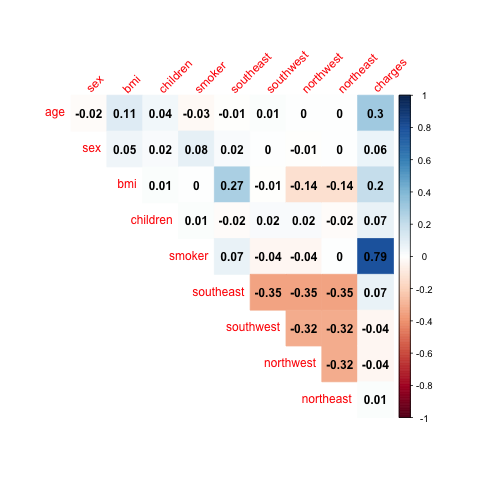
\includegraphics[width=0.75\linewidth,height=0.75\textheight]{C:/Users/nimad/Downloads/STAT 547/Project/group_01_dlin_njamshidi-1/images/corrplot} 

}

\caption{Correlation plot}\label{fig:corrplot-png}
\end{figure}

In order to to check if there is any cluster of data points, we use faceted plot (Figure \ref{fig:facet-png}). While the data between regions and sex does not appear to vary much, the smokers vs nonsmokers of each facet appear to cluster together, with the non-smokers having an overall lower medical cost.

\begin{figure}

{\centering 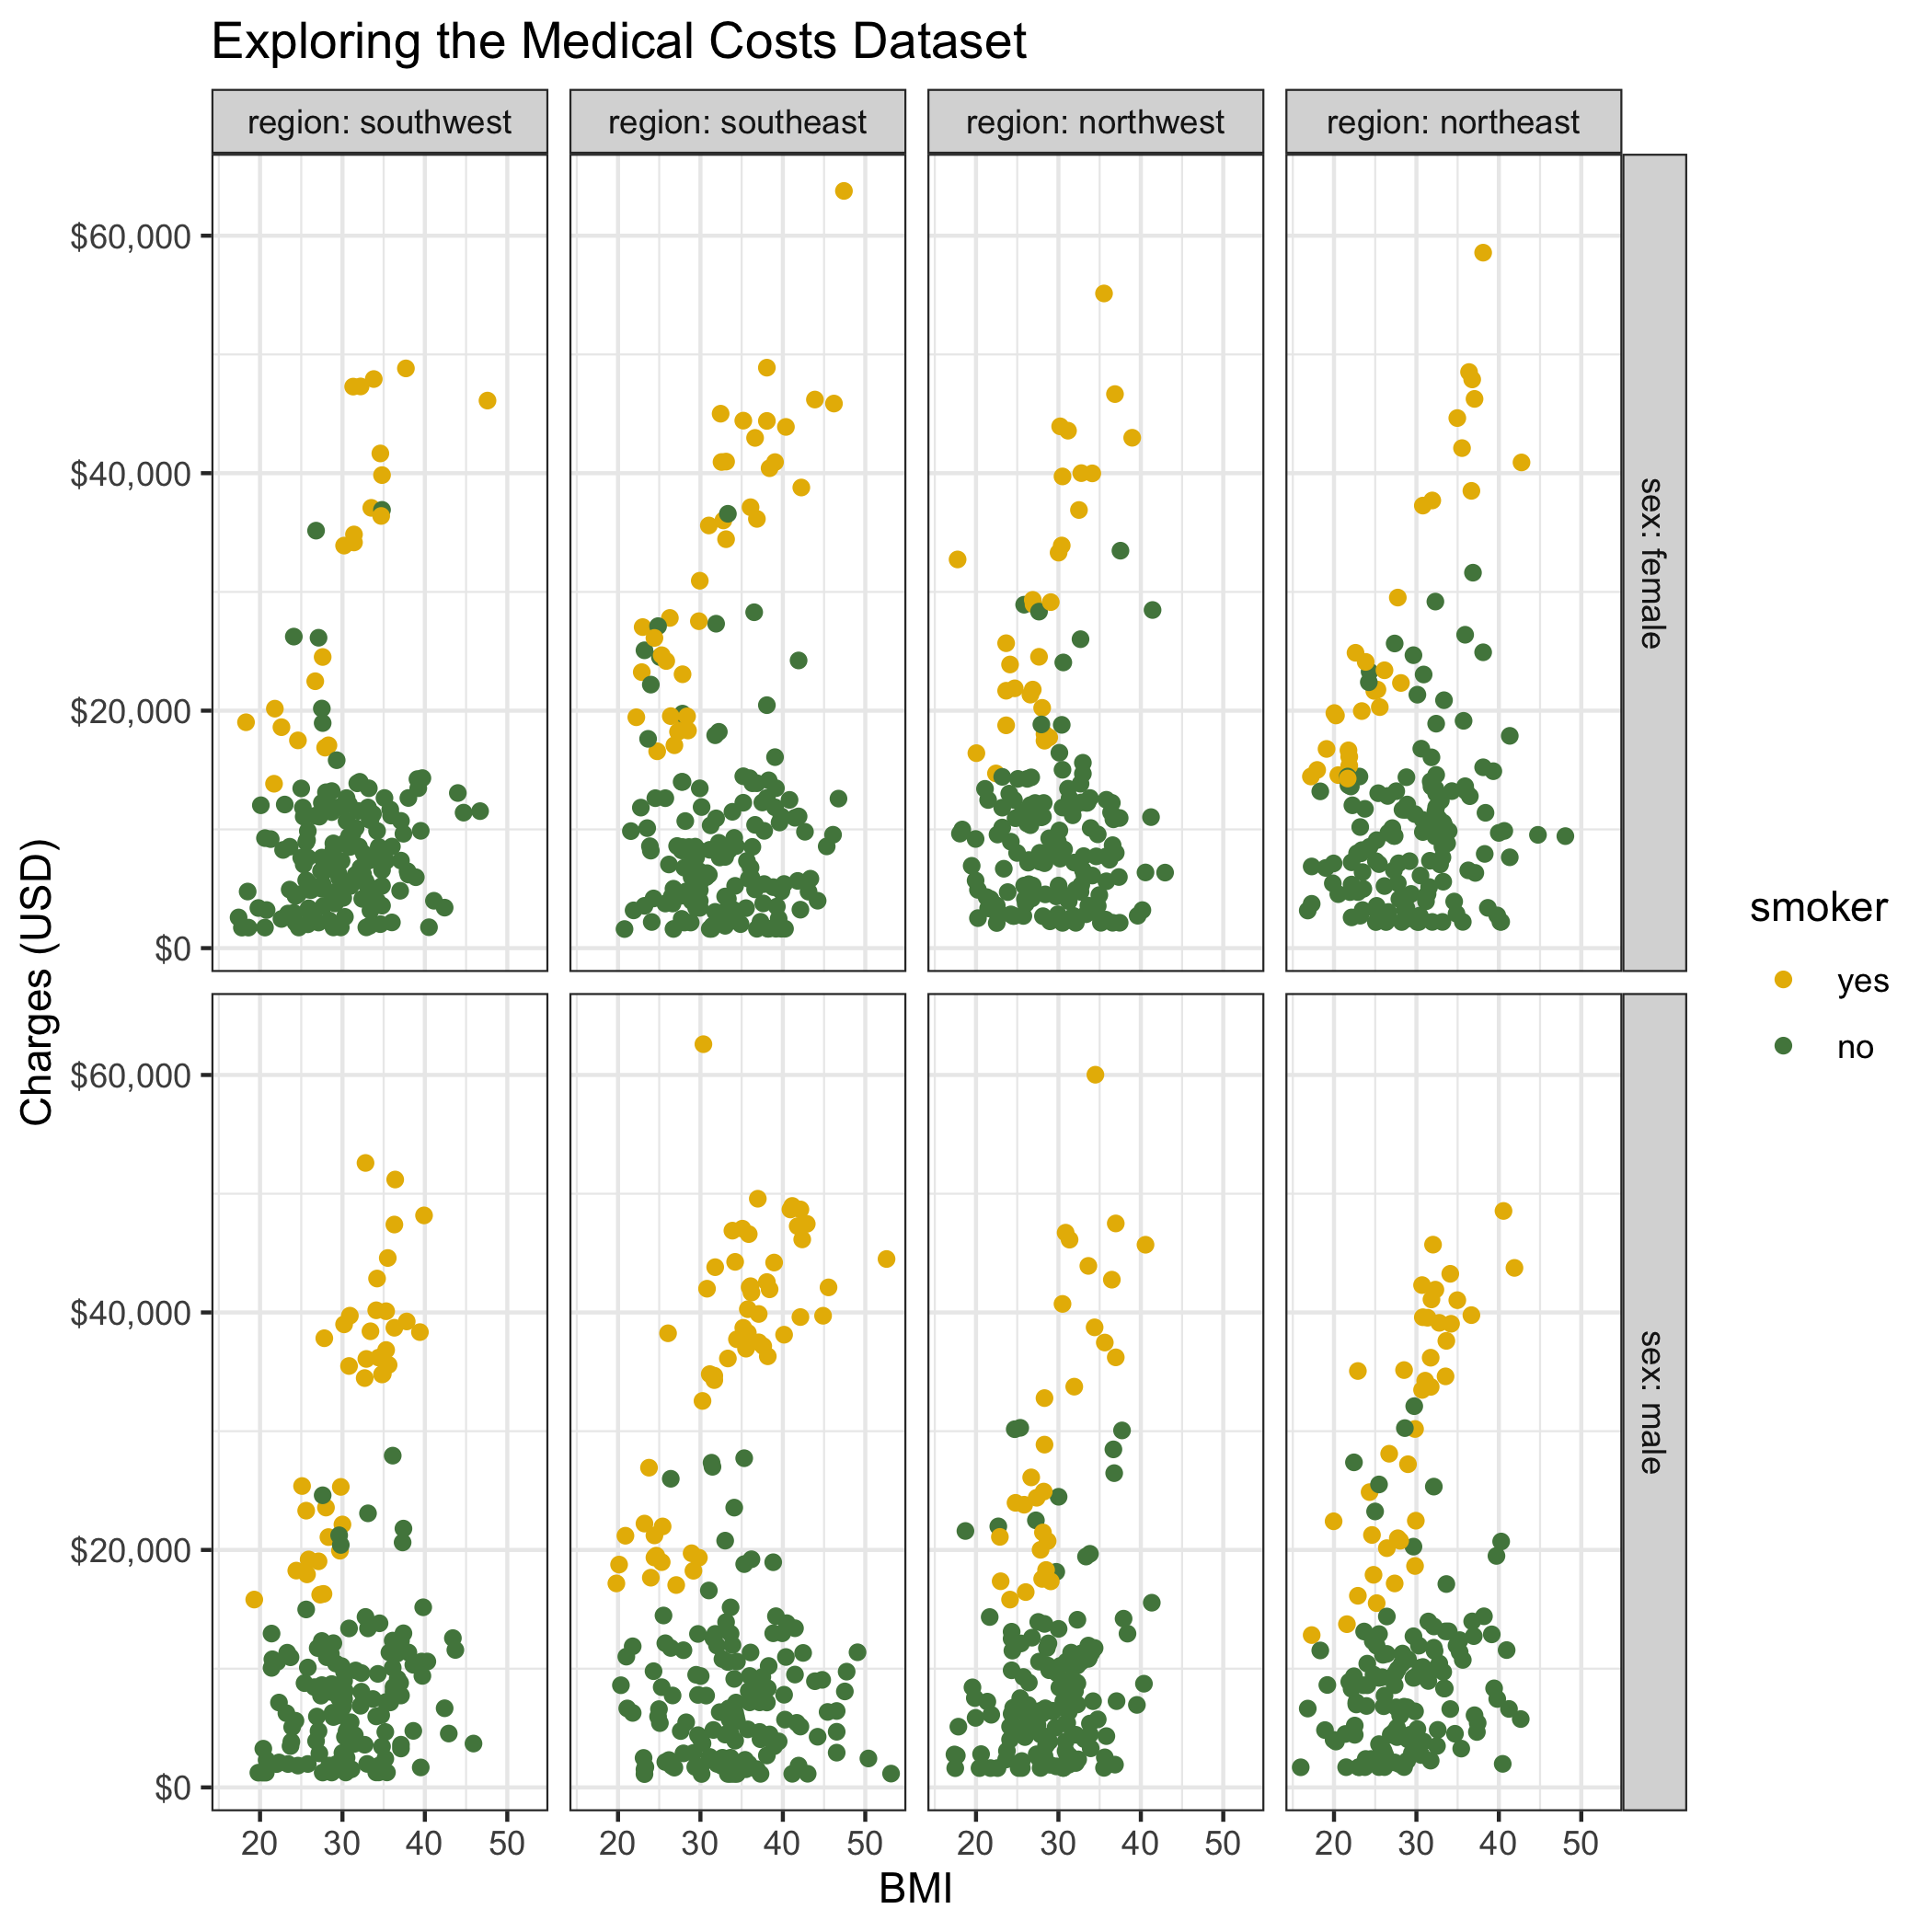
\includegraphics[width=0.75\linewidth,height=0.75\textheight]{C:/Users/nimad/Downloads/STAT 547/Project/group_01_dlin_njamshidi-1/images/facet} 

}

\caption{Exploring the medical costs dataset}\label{fig:facet-png}
\end{figure}

How is the distribution of sex among different age groups?
Looking at Figure \ref{fig:agehist-png}, there appears to be more beneficiaries in the 20-60 age range. The biggest difference in the number of beneficiaries from different sex is seen in the 20-30 bracket.

\begin{figure}

{\centering 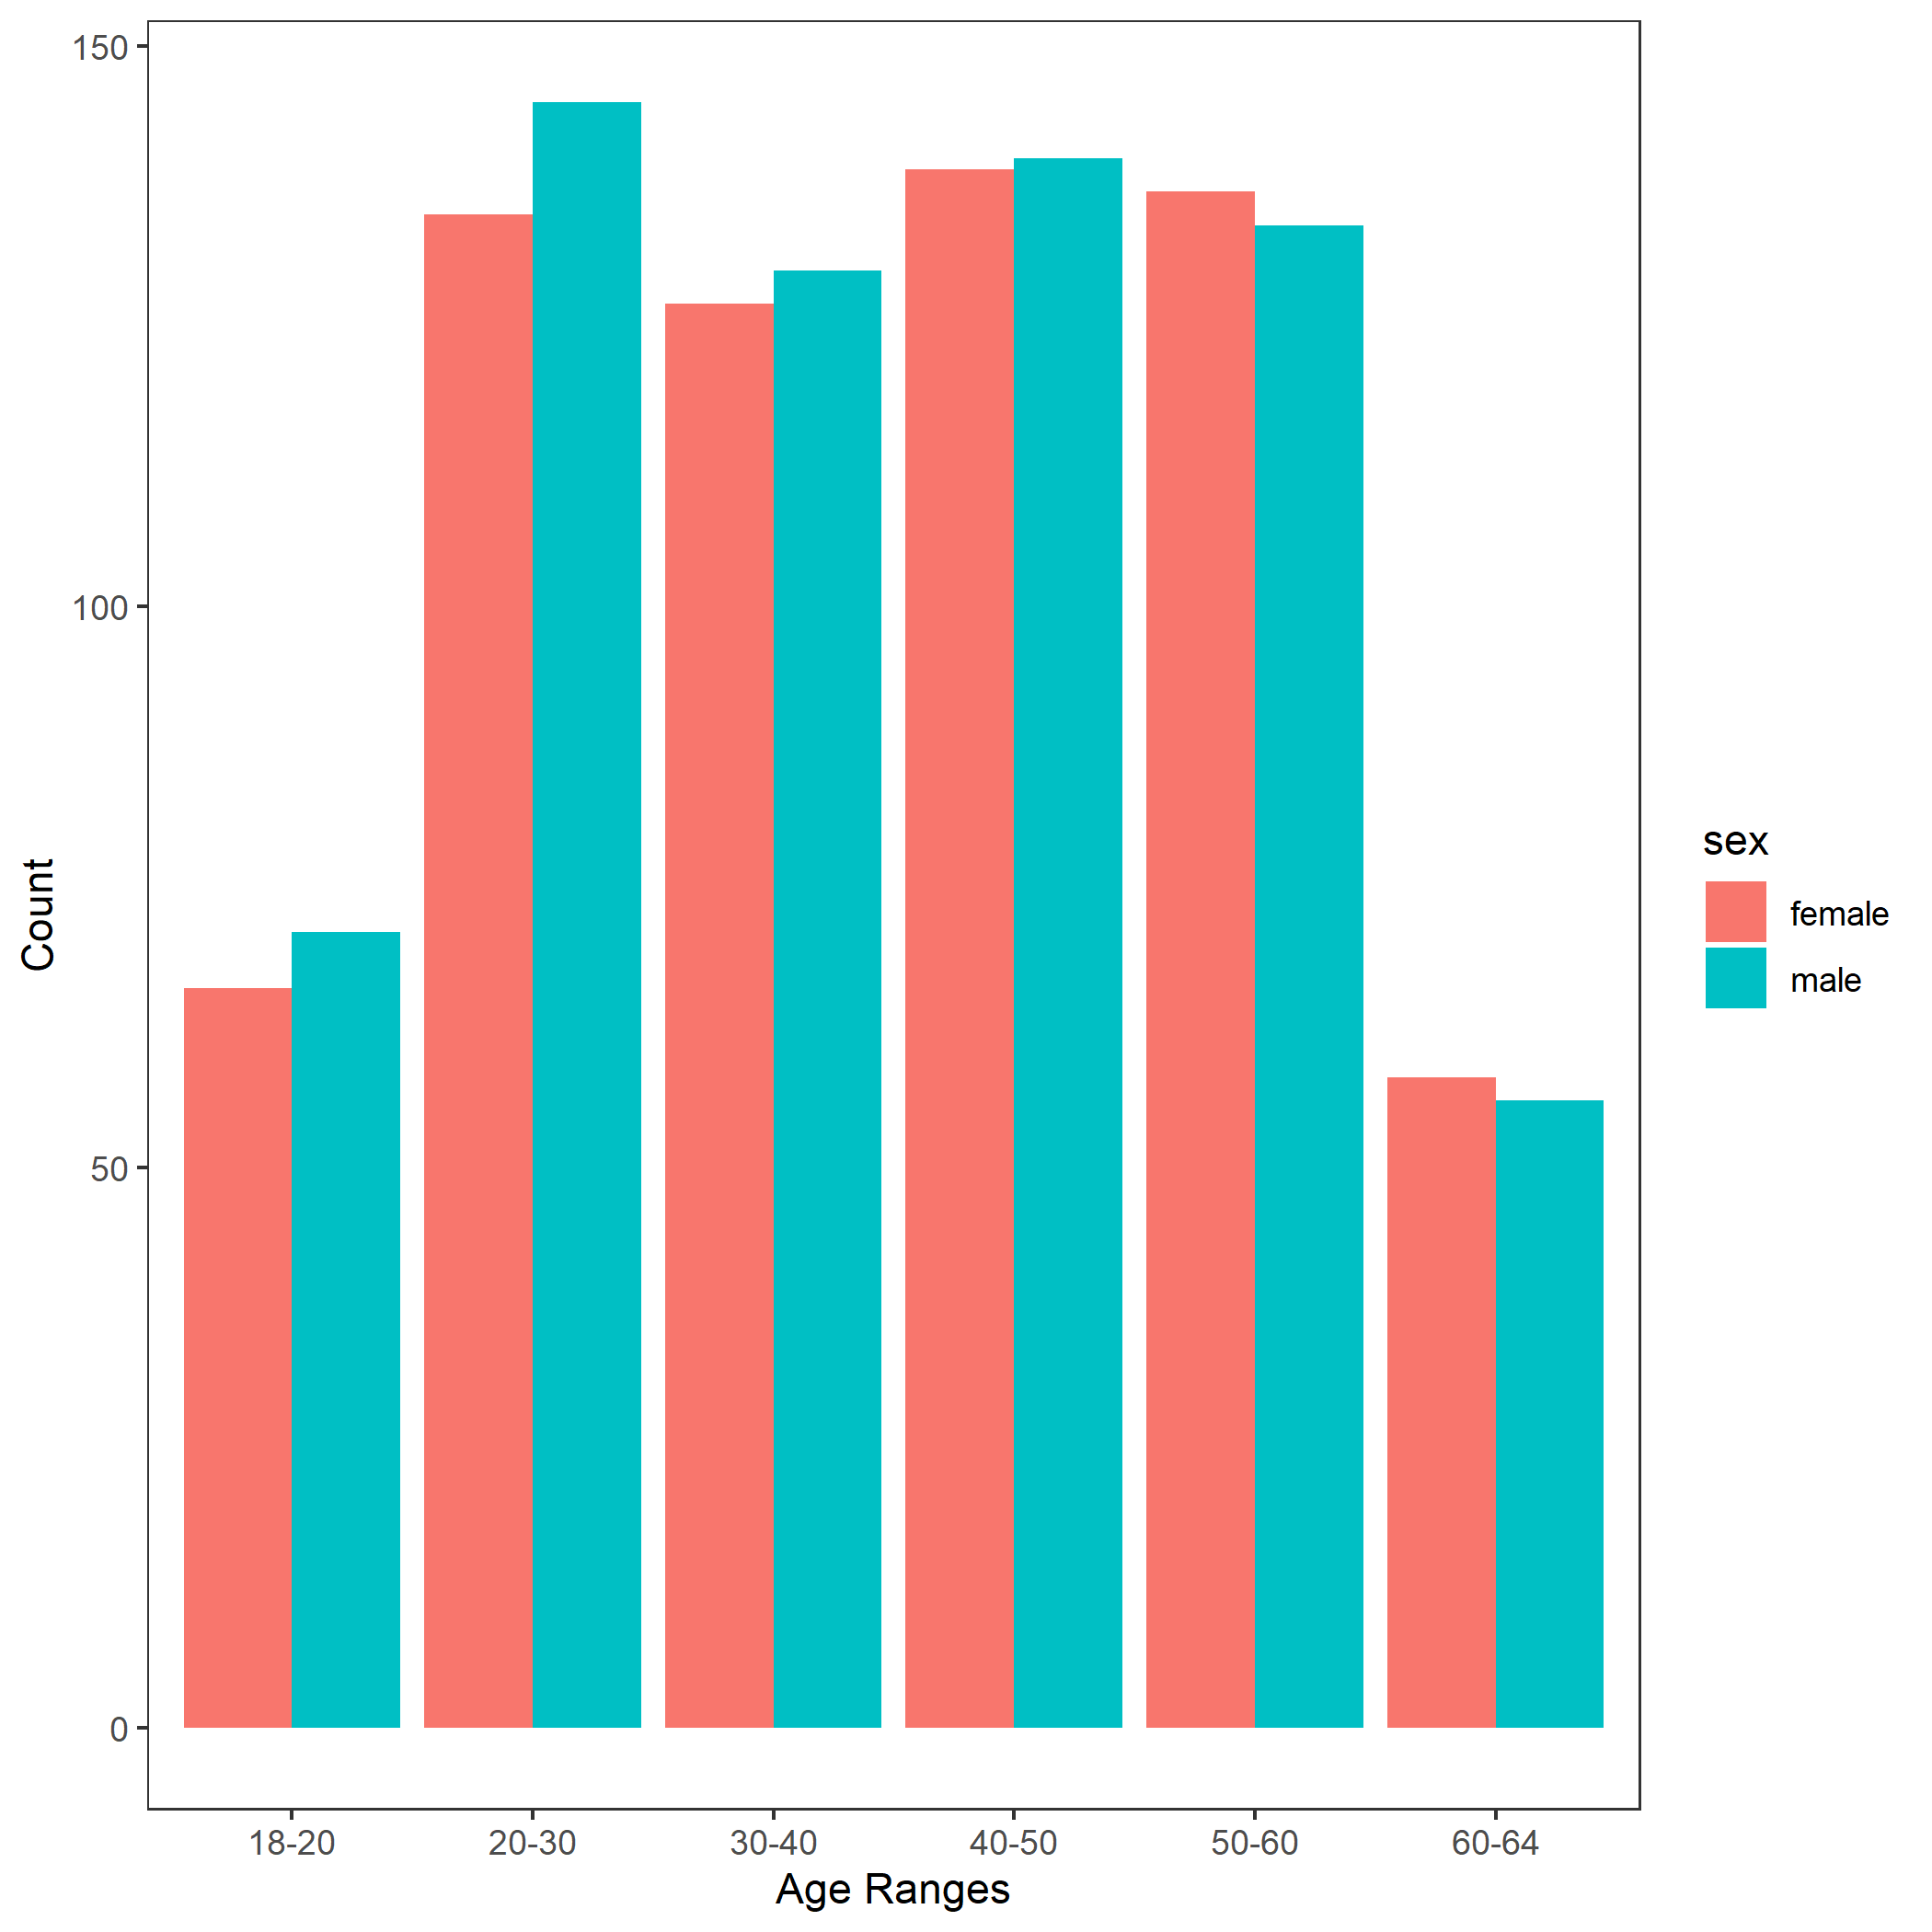
\includegraphics[width=0.75\linewidth,height=0.75\textheight]{C:/Users/nimad/Downloads/STAT 547/Project/group_01_dlin_njamshidi-1/images/age_histogram} 

}

\caption{Distribution of age ranges}\label{fig:agehist-png}
\end{figure}

How about the distribution of sex among the regions?
Figure \ref{fig:barplot-png} shows the distribution of sex in each of the four regions. At a glance, the dataset looks very even when it comes to sex, but there are slightly more beneficiaries in the southeast.

\begin{figure}

{\centering 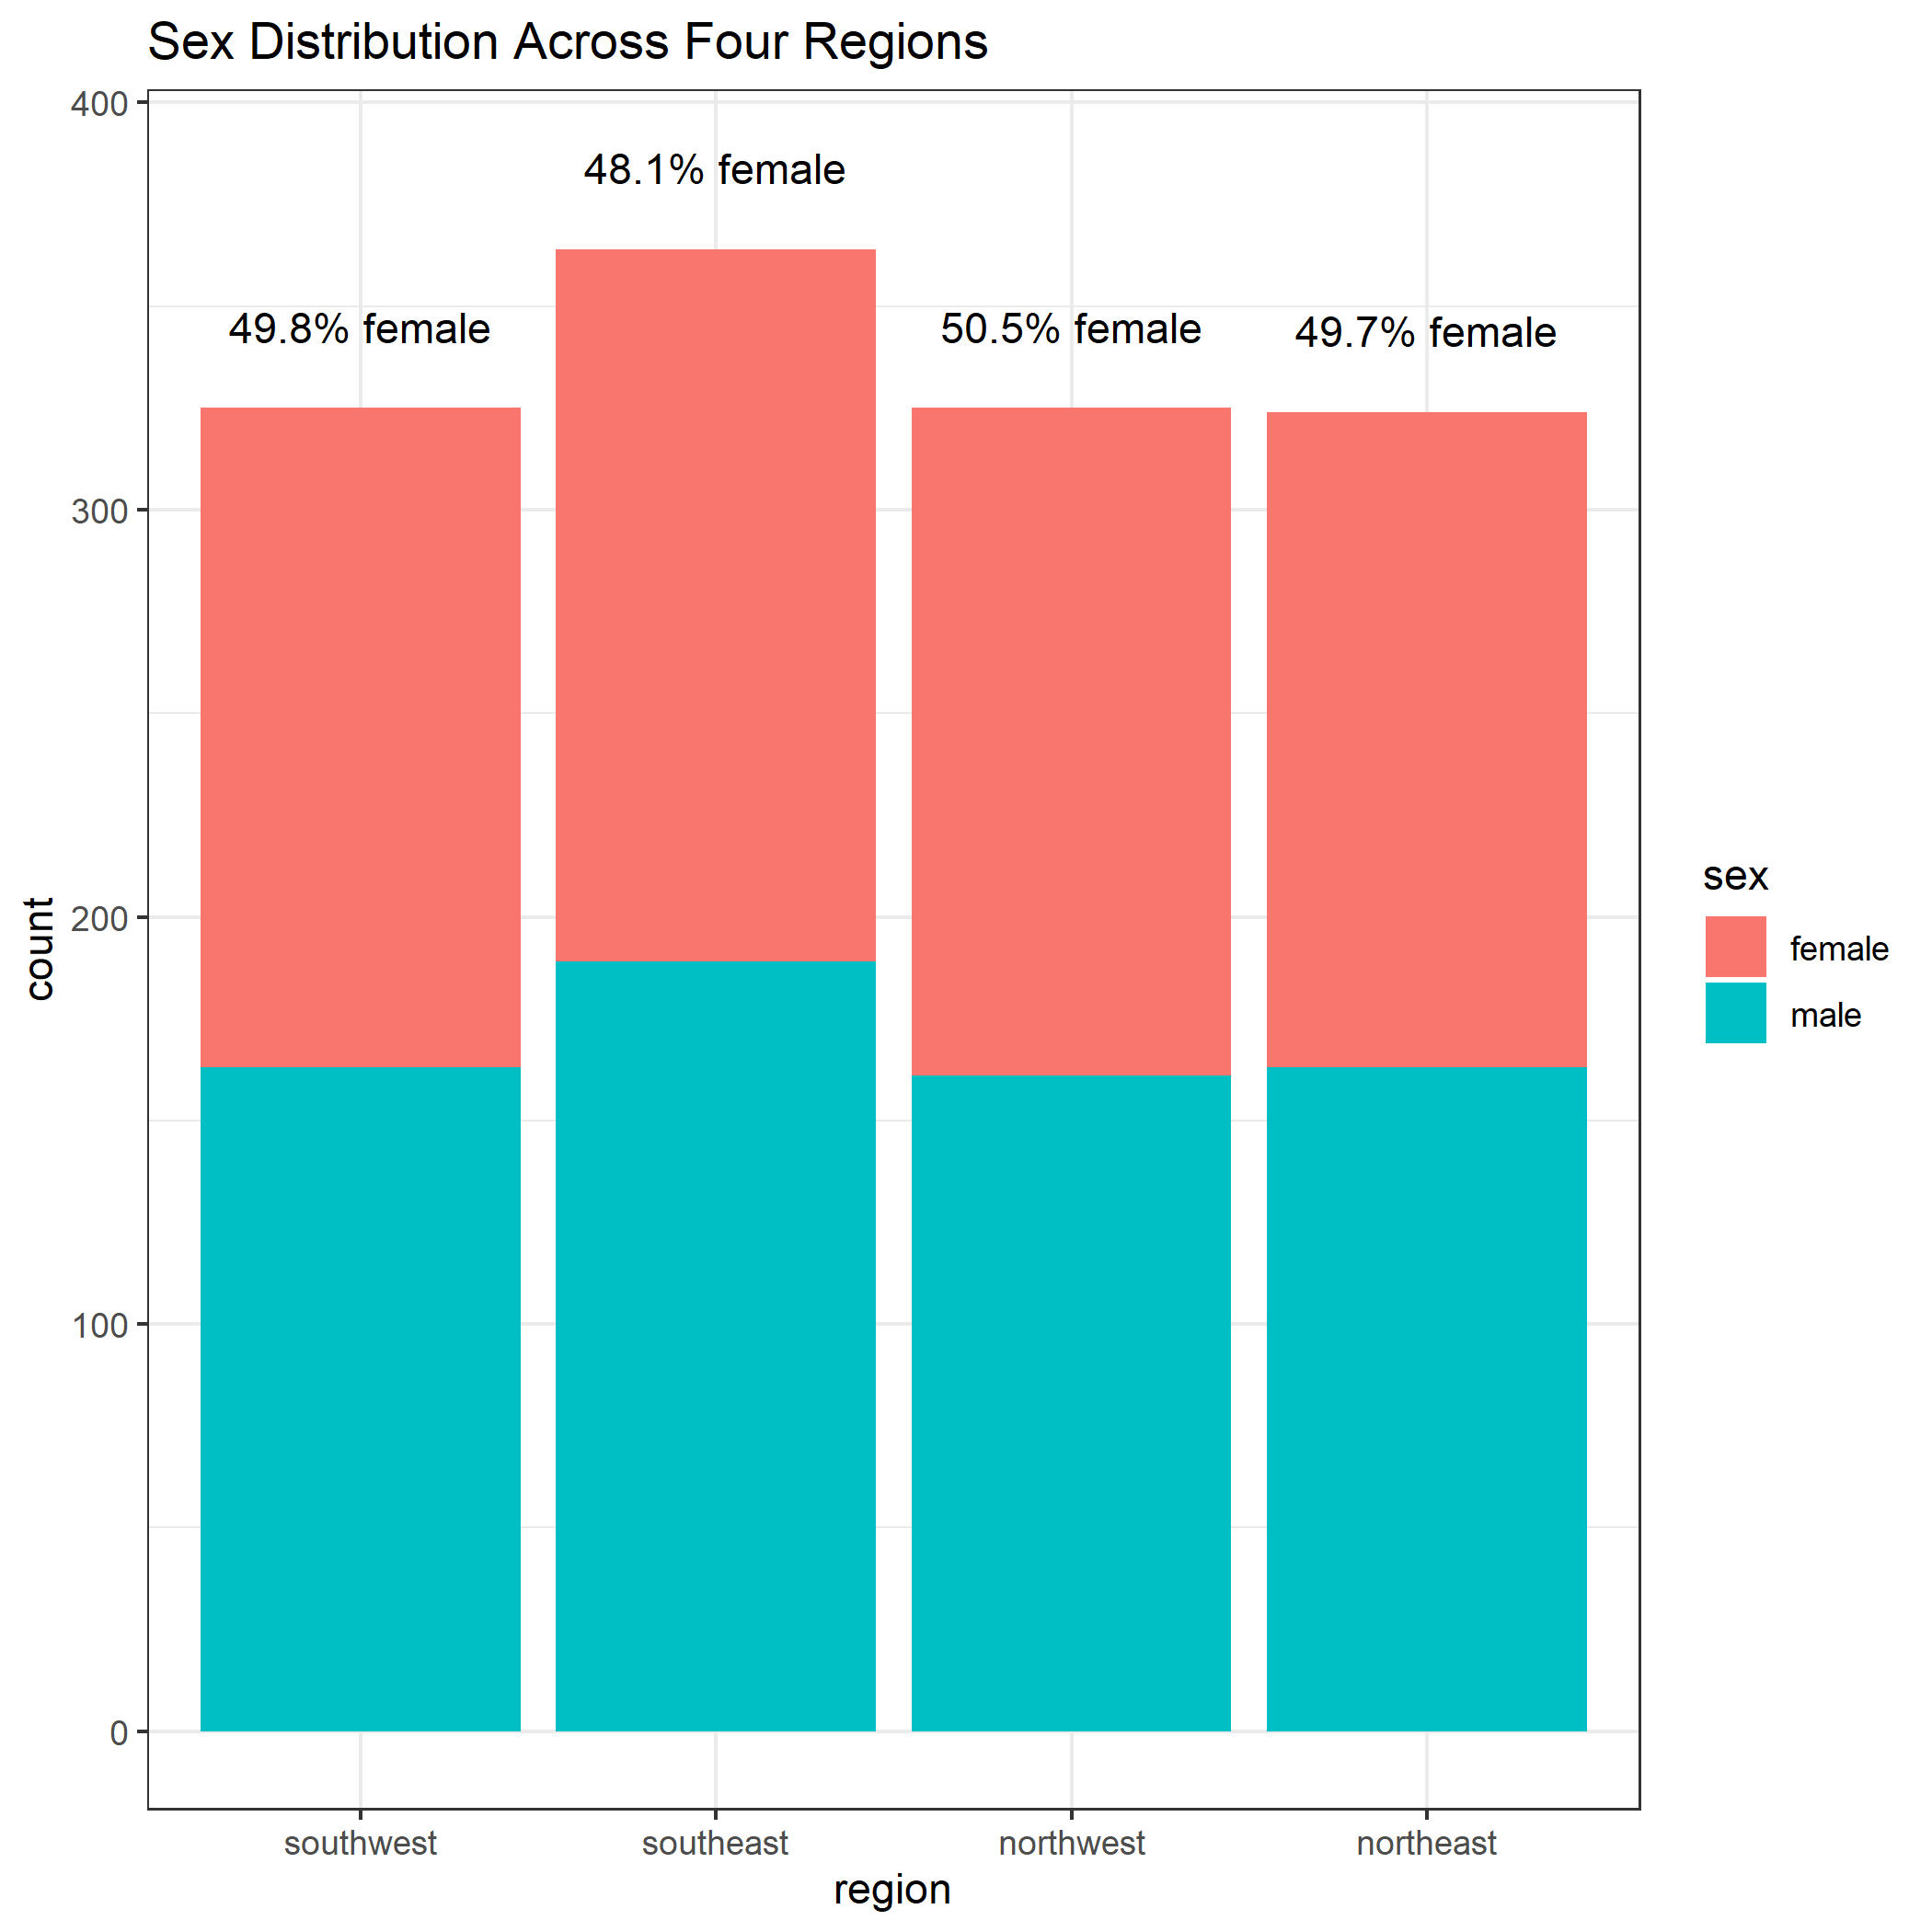
\includegraphics[width=0.75\linewidth,height=0.75\textheight]{C:/Users/nimad/Downloads/STAT 547/Project/group_01_dlin_njamshidi-1/images/region_barchart} 

}

\caption{Sex distribution across four regions}\label{fig:barplot-png}
\end{figure}

\hypertarget{methods}{%
\section{Methods}\label{methods}}

Here we use multiple linear regression to study the relations between the independent variables and the dependent one, charges. Below you can find the results of the regression in Table \ref{tab:methods-tidy}. \texttt{lm} function in R transforms a categorical variable with n levels into n-1 variables each with two levels to insure the variables are independent. Here we can see that varables age, bmi, children, and smoker are significantly important in the regression. Sex is an insignificant factor in the model.

\begin{table}

\caption{\label{tab:methods-tidy}Summary of the model's variables and their respective coefficients}
\centering
\begin{tabular}[t]{l|r|r|r|r}
\hline
term & estimate & std.error & statistic & p.value\\
\hline
(Intercept) & -11938.5386 & 987.81918 & -12.0857530 & 0.0000000\\
\hline
age & 256.8564 & 11.89885 & 21.5866552 & 0.0000000\\
\hline
sexmale & -131.3144 & 332.94544 & -0.3944020 & 0.6933475\\
\hline
bmi & 339.1935 & 28.59947 & 11.8601306 & 0.0000000\\
\hline
children & 475.5005 & 137.80409 & 3.4505546 & 0.0005770\\
\hline
smokeryes & 23848.5345 & 413.15335 & 57.7232020 & 0.0000000\\
\hline
regionnorthwest & -352.9639 & 476.27579 & -0.7410914 & 0.4587689\\
\hline
regionsoutheast & -1035.0220 & 478.69221 & -2.1621870 & 0.0307817\\
\hline
regionsouthwest & -960.0510 & 477.93302 & -2.0087563 & 0.0447649\\
\hline
\end{tabular}
\end{table}

In Table \ref{tab:methods-glance} we can see that the r-squared value is 0.75. Figure \ref{fig:regression} shows the diagnostics plots of the regression model.

\begin{table}

\caption{\label{tab:methods-glance}Model summary}
\centering
\begin{tabular}[t]{r|r|r|r|r|r|r|r|r|r|r}
\hline
r.squared & adj.r.squared & sigma & statistic & p.value & df & logLik & AIC & BIC & deviance & df.residual\\
\hline
0.750913 & 0.7494136 & 6062.102 & 500.8107 & 0 & 9 & -13547.75 & 27115.51 & 27167.5 & 48839532844 & 1329\\
\hline
\end{tabular}
\end{table}

\begin{figure}

{\centering 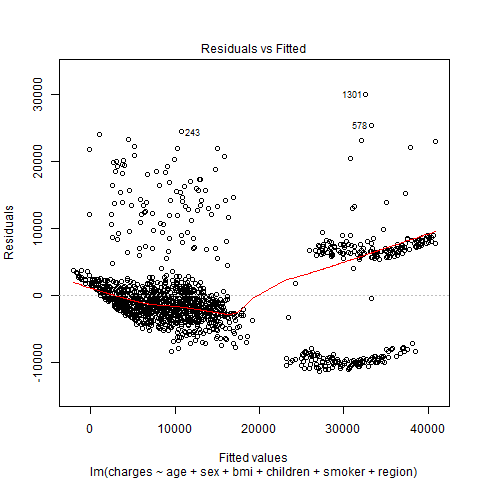
\includegraphics[width=0.49\linewidth,height=0.2\textheight]{C:/Users/nimad/Downloads/STAT 547/Project/group_01_dlin_njamshidi-1/images/lmplot001} 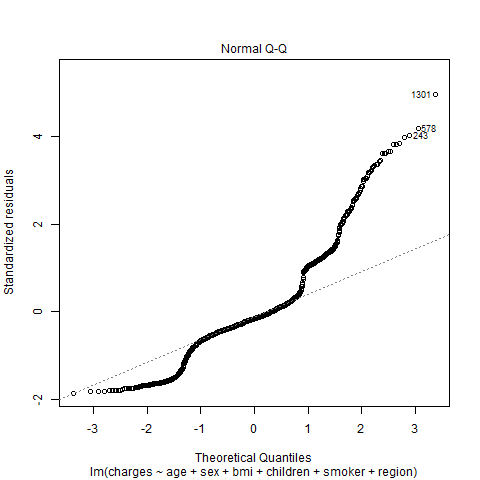
\includegraphics[width=0.49\linewidth,height=0.2\textheight]{C:/Users/nimad/Downloads/STAT 547/Project/group_01_dlin_njamshidi-1/images/lmplot002} 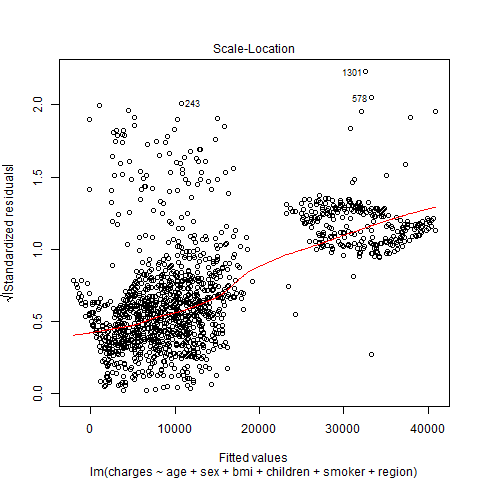
\includegraphics[width=0.49\linewidth,height=0.2\textheight]{C:/Users/nimad/Downloads/STAT 547/Project/group_01_dlin_njamshidi-1/images/lmplot003} 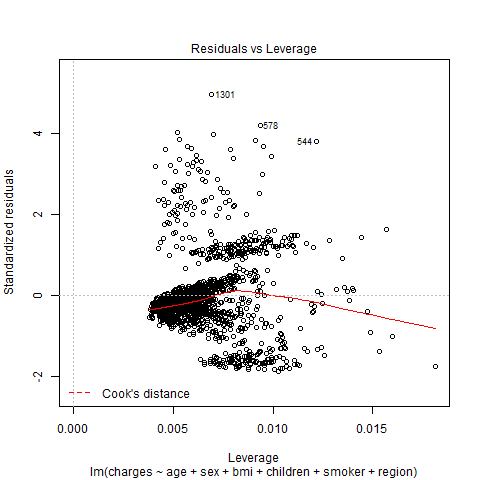
\includegraphics[width=0.49\linewidth,height=0.2\textheight]{C:/Users/nimad/Downloads/STAT 547/Project/group_01_dlin_njamshidi-1/images/lmplot004} 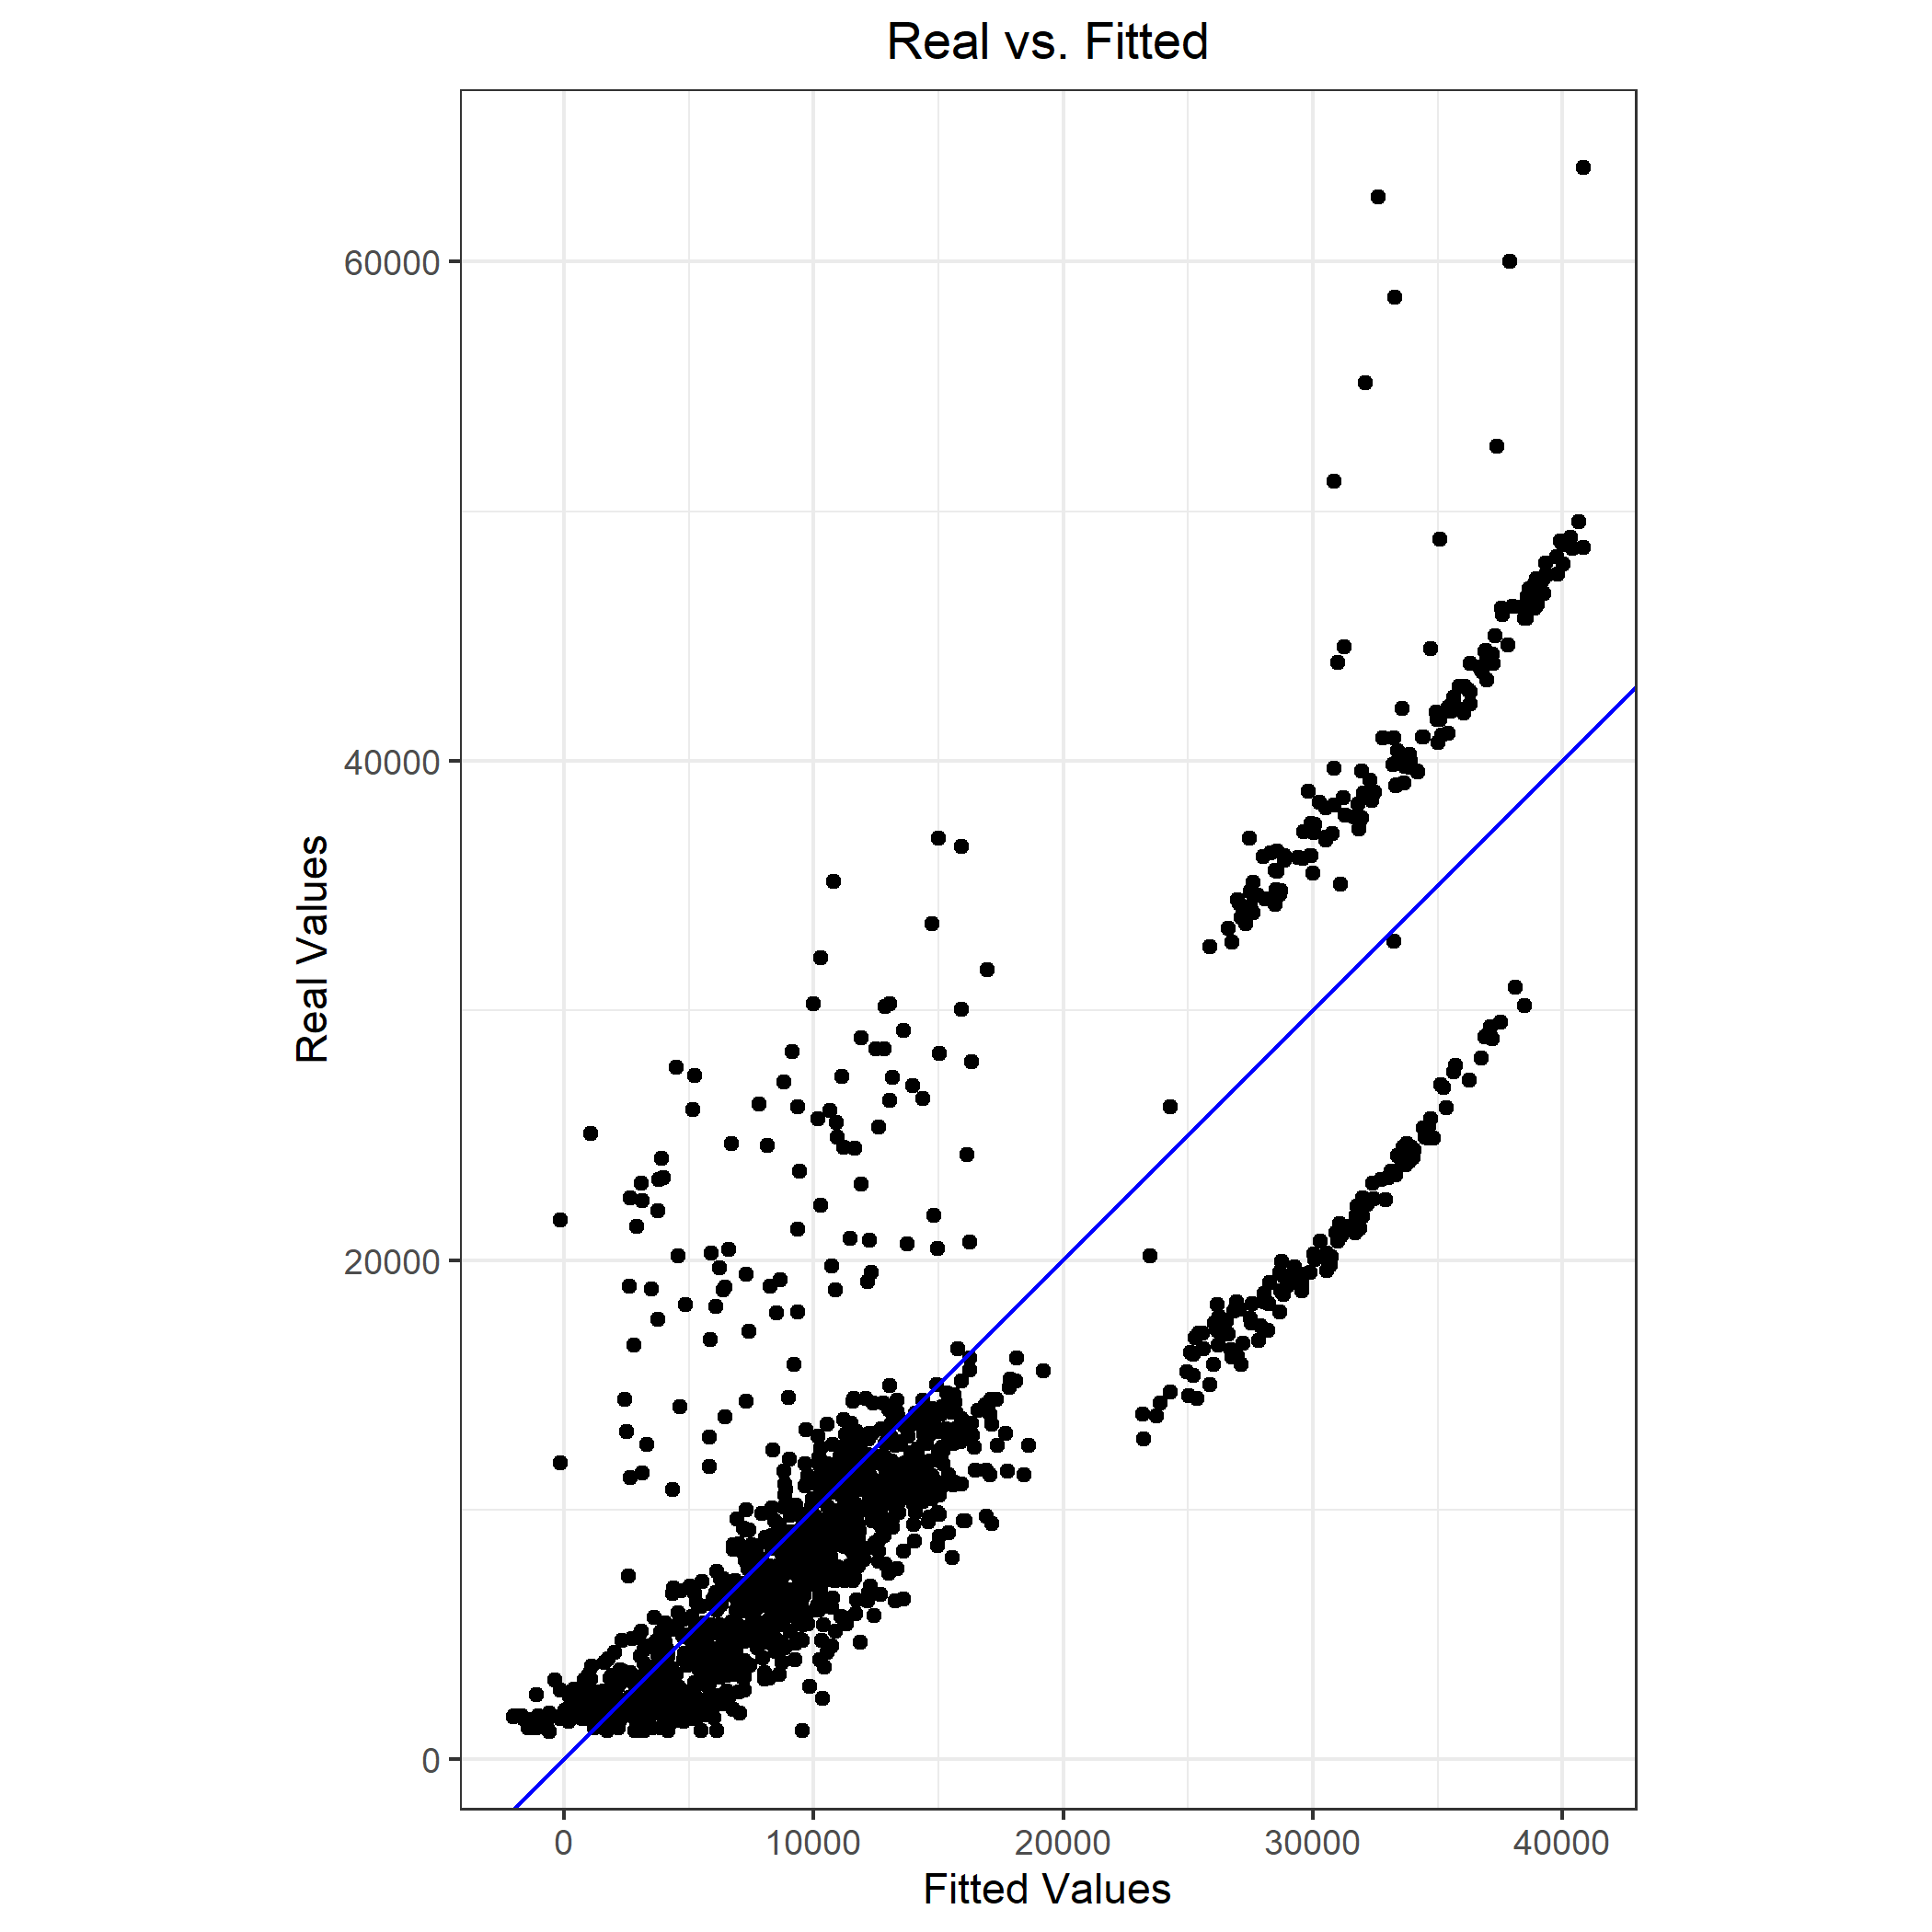
\includegraphics[width=0.49\linewidth,height=0.2\textheight]{C:/Users/nimad/Downloads/STAT 547/Project/group_01_dlin_njamshidi-1/images/lmplot005} 

}

\caption{regression diagnostics plots}\label{fig:regression}
\end{figure}

\hypertarget{results}{%
\section{Results}\label{results}}

In Table \ref{tab:results} you can find a number of examples of the data with their fitted value.

\begin{table}

\caption{\label{tab:results}Estimated values their statistics}
\centering
\begin{tabular}[t]{r|r|l|r|r|l|l|r|r|r|r|r|r|r}
\hline
charges & age & sex & bmi & children & smoker & region & .fitted & .se.fit & .resid & .hat & .sigma & .cooksd & .std.resid\\
\hline
16884.924 & 19 & female & 27.900 & 0 & yes & southwest & 25293.713 & 586.0725 & -8408.7890 & 0.0093467 & 6059.951 & 0.0020361 & -1.3936360\\
\hline
1725.552 & 18 & male & 33.770 & 1 & no & southeast & 3448.603 & 448.8438 & -1723.0505 & 0.0054821 & 6064.199 & 0.0000498 & -0.2850155\\
\hline
4449.462 & 28 & male & 33.000 & 3 & no & southeast & 6706.988 & 480.0578 & -2257.5265 & 0.0062711 & 6064.066 & 0.0000979 & -0.3735731\\
\hline
21984.471 & 33 & male & 22.705 & 0 & no & northwest & 3754.830 & 460.7247 & 18229.6404 & 0.0057761 & 6043.597 & 0.0058713 & 3.0158709\\
\hline
3866.855 & 32 & male & 28.880 & 0 & no & northwest & 5592.493 & 424.3699 & -1725.6382 & 0.0049005 & 6064.198 & 0.0000446 & -0.2853601\\
\hline
3756.622 & 31 & female & 25.740 & 0 & no & southeast & 3719.826 & 454.5231 & 36.7958 & 0.0056217 & 6064.384 & 0.0000000 & 0.0060869\\
\hline
\end{tabular}
\end{table}

\hypertarget{discussion}{%
\section{Discussion}\label{discussion}}

Based on the ``Residuals vs Fitted'' and ``Real vs Fitted'' graphs, we can see that the model fairly works for charges under 2000\$. There are three clusters in these graphs with similar slopes. There is a gap between charges under and over 2000\$ which might be relevant to the weak estimates of the model over 2000\$.
If we apply linear regression on each cluster we will get similar coefficients for the variables with different intercepts. Each cluster might be attributed to a different desease group and in each of them the impacts of age, smoking, bmi and etc. are similar.

\hypertarget{conclusion}{%
\section{Conclusion}\label{conclusion}}

We were able to do a linear regression on our dataset. The results show that there is an association relationship between age, bmi, number of children, and smoking with medical charges. interestingly, gender does not affect medical charges. Diagnostic plots reveal that the data is not completely normally distributed. Moreover, three clusters of records are present in the dataset, which might be representative of different types of deseases.

\end{document}
